\section{Statistics}

\subsection{Correlation}
Assume an inner product space.

\subsection{Linear regression}

Assume that reality can me modelled by a model like this one: 

$$ \vec{y} = \mtrx{X} \vec{w} + \vec{e} $$

Not knowing $\vec{e}$, our best guess at the outcome would be 

$$ \vec{\hat{y}} = \mtrx{X} \vec{w} $$

We can find the gradient of w by:

$$ \partDiff{E}{\vec{w}} = -  (\vec{y} - \vec{\hat{y}}) \mtrx{X}  $$



\subsection{Spatial modelling}

\subsubsection{Generalized least squares}
like linear regression, but errors are not iid, but allowed to be correlated.

\subsubsection{Gaussian processes}
Gaussian processes are a means of interpolating a value $y_x$ from surrounding values $y_x = \sum \alpha_i y_i$. Basic intuition from \href{https://bookdown.org/rbg/surrogates/chap5.html}{here}.
That is different from what linear regression or its extension GLS do: regression predicts $y$ from explanatory variables $x$, assuming a (linear) model.
Gaussian processes don't do that. They only interpolate between already observed $y$'s. No model is assumed.

Consider the $n \times m$ surface $\mtrx{Y}$. Assume that the value of any pixel in $\mtrx{Y}$ follows a gaussian distribution - which may be correlated to all other pixels in $\mtrx{Y}$.
Millions of surfaces $\mtrx{Y}$ may be sampled from $N(\vec{0}, \mtrx{\Sigma}) = P(\mtrx{Y})$, where $\vec(0)$ is of size $n \times m$ and $\mtrx{\Sigma}$ is of size $nm \times nm$.
We call $P(\mtrx{Y})$ the prior. $\mtrx{\Sigma}$ can be very large, so we assume that it can be modeled by a covariance-function $cov(h)$ which is \emph{only dependent on the distance between two points, not on the points themselves}.

\begin{lstlisting}[language=python]
import numpy as np
import matplotlib.pyplot as plt
from scipy.stats import multivariate_normal

def size(x):
    return np.sqrt(np.sum(np.power(x, 2)))

def distance(x0, x1):
    return size(x0 - x1)

def getDistanceMatrix(rowPoints, colPoints):
    # deliberately not exploiting symmetry 
    # <- this way it works with non-square matrices, too.
    rows = len(rowPoints)
    cols = len(colPoints)
    distances = np.zeros((rows, cols))
    for i in range(rows):
        for j in range(cols): 
            p0 = rowPoints[i]
            p1 = colPoints[j]
            d = distance(p0, p1)
            distances[i, j] = d
    return distances

deltaX = 0.1
deltaY = 0.1
gridX = 20
gridY = 20
nrPoints = gridX * gridY
points = np.zeros((nrPoints, 2))
for x in range(gridX):
    for y in range(gridY):
        i = x * gridX + y
        points[i] = [x * deltaX, y * deltaY]
distances = getDistanceMatrix(points, points)

mean = np.zeros((nrPoints))
cov0 = 1.3  # overall variance
h95 = 2     # distance at which cov(h) >= 0.95 * cov0

def variogramFunction(h):
    return cov0 * ( 1 - np.exp( -3*h/h95 ) )

Sigma = cov0 - variogramFunction(distances)
prior = multivariate_normal(mean, Sigma)

sample1 = prior.rvs()
sample2 = prior.rvs()
sample3 = prior.rvs()
\end{lstlisting}

\begin{figure}[H]
    \caption{3 samples from prior $P(\mtrx{Y})$}
    \centering
    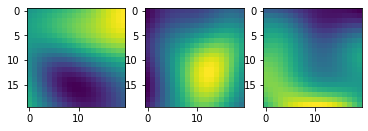
\includegraphics[width=0.7\linewidth]{images/gp_prior_samples.png}
\end{figure}

We have observed some samples $\mtrx{D} = {(x_i, y_i)}$.
Which of these millions of surfaces are most likely given those observations? We can answer that with $P(\mtrx{Y}|\mtrx{D})$.
\begin{figure}[H]
    \caption{Observations $\mtrx{D}$. Which field $\mtrx{Y}$ is most likely to have produced these observations?}
    \centering
    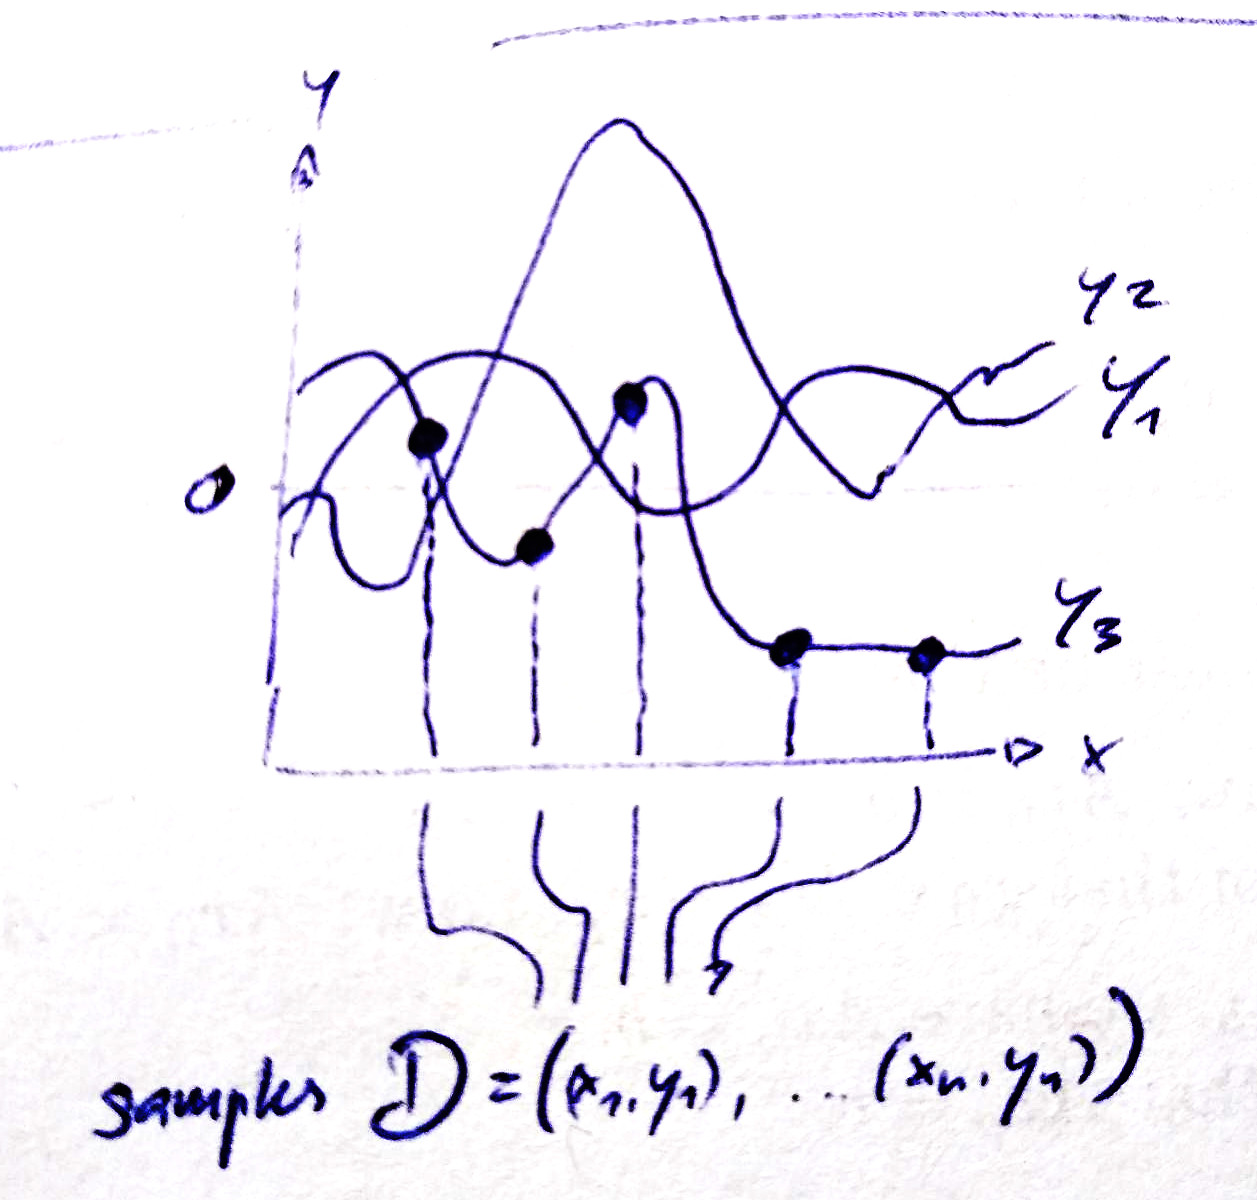
\includegraphics[width=0.4\linewidth]{images/gp_observations.jpg}
\end{figure}

We can calculate the posterior using 
$$
P(\mtrx{Y}|\mtrx{D}) \sim P(\mtrx{D}|\mtrx{Y}) P(\mtrx{Y})
$$
But since in gaussian processes we assume multivariate-normals, this can be done much easier.

Consider a multivariate normal distribution on, say, 400 dimensions $N(\vec{\mu}, \mtrx{\Sigma})$. Those 400 dimensions could, for example, be pixel-values in a 20 by 20 image.
Now assume that out of those 400 dimensions we have measurements for $s$ samples, leaving a rest $r = 400 - s$.
For multivariate-normal distributions, we can easily and analytically obtain the conditional distribution $P(\vec{y}_r | \vec{y}_s) = N(\hat{\vec{\mu}}, \hat{\mtrx{\Sigma}})$.

Split $\vec{y}$ like so:
$$ y = \myarray{\vec{y}_r \\ \vec{y}_s} $$
Analogously we can split the covariance-matrix:
$$ \mtrx{\Sigma} = \begin{bmatrix}
    \mtrx{\Sigma}_{rr} & \mtrx{\Sigma}_{rs} \\
    \mtrx{\Sigma}_{sr} & \mtrx{\Sigma}_{ss} \\
\end{bmatrix}  $$

Then, according to \href{https://en.wikipedia.org/wiki/Multivariate_normal_distribution#Conditional_distributions}{wikipedia}, we can obtain $\hat{\vec{\mu}}$ and $\hat{\mtrx{\Sigma}}$ like so:
$$ \hat{\vec{\mu}}_r = \vec{\mu}_r + \mtrx{\Sigma}_{rs} \mtrx{\Sigma}_{ss}^{-1} (\vec{y}_s - \vec{\mu}_s) $$
$$ \hat{\mtrx{\Sigma}}_r = \mtrx{\Sigma}_{rr} - \mtrx{\Sigma}_{rs} \mtrx{\Sigma}_{ss}^{-1} \mtrx{\Sigma}_{sr} $$

\begin{lstlisting}[language=python]
indices = np.arange(nrPoints)
sampleIndices = np.asarray(list(
    map(lambda x: int(x),
        samples[:, 0])))
nonSampleIndices = np.asarray(list(
    filter(lambda v: v not in sampleIndices,
           indices)))
samplePoints = points[sampleIndices]
nonSamplePoints = points[nonSampleIndices]
sampleValues = samples[:, 3]

# For simplicity, we just re-calculate SigmaXX here.
# But we could have also picked the right values from Sigma
# without any need for re-computation.
distancesRR = getDistanceMatrix(nonSamplePoints, nonSamplePoints)
SigmaRR = cov0 - variogramFunction(distancesRR)

distancesSS = getDistanceMatrix(samplePoints, samplePoints)
SigmaSS = cov0 - variogramFunction(distancesSS)
SigmaSSInverse = np.linalg.inv(SigmaSS)

distancesRS = getDistanceMatrix(nonSamplePoints, samplePoints)
SigmaRS = cov0 - variogramFunction(distancesRS)
SigmaSR = SigmaRS.transpose()

meanPosterior = SigmaRS @ SigmaSSInverse @ sampleValues
SigmaPosterior = SigmaRR - SigmaRS @ SigmaSSInverse @ SigmaSR

posterior = multivariate_normal(meanPosterior, SigmaPosterior)   
\end{lstlisting}

We can now plot the \inlinecode{meanPosterior} around our \inlinecode{samples}. Doing so we obtain the graphic as shown in figure \ref{gpPosterior}.

\begin{figure}[H]
  \centering
  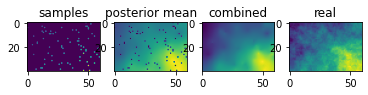
\includegraphics[width=0.7\linewidth]{images/gp_posterior_samples.png}
  \caption{Samples and fitted posterior fit together well}
  \label{gpPosterior}
\end{figure}


Note how we assumed that the covariance matrix $\mtrx{\Sigma}$ could be parameterized with a covariance-function $c(h)$. Only this way do we have any chance of finding a good approximation for $\mtrx{\Sigma}$ with only few samples.
The relation \inlinecode{Sigma = cov0 - variogramFunction(distances)} comes from the variogram $\gamma(h)$ as in here:
\begin{equation}
  \begin{aligned}
    2 \gamma(h) &= E[(Z(x+h) - Z(x))^2] \\
                &= E[( (Z(x+h) - \mu) - (Z(x) - \mu) )^2] \\
                &= E[ (Z(x+h) - \mu)^2  - 2(Z(x+h) - \mu)(Z(x) - \mu)  + (Z(x) - \mu)^2 ] \\
                &= E[ (Z(x+h) - \mu)^2 ]  - 2 E[(Z(x+h) - \mu)(Z(x) - \mu)]  + E[ (Z(x) - \mu)^2 ] \\
                &= c(0) - 2 c(h) + c(0) \\
      \gamma(h) &= c(0) - c(h) \\
           c(h) &= c(0) - \gamma(h)
  \end{aligned}
\end{equation}
In practical applications, we'll usually fit our function \inlinecode{cov0 * ( 1 - np.exp( -3*h/h95 ) )} by moving the parameters \inlinecode{cov0} and \inlinecode{h95} until the residuals fit properly.
Our code would then look like this:

\begin{lstlisting}[language=python]
def empiricalVariogram(distanceMatrix, data):
  variogram = {}
  d0 = np.min(distanceMatrix)
  d1 = np.max(distanceMatrix)
  nrHs = 20
  deltaH = (d1 - d0) / nrHs
  for h in np.linspace(d0, d1, nrHs):
      Nh = 0
      hSum = 0
      pairs = (h <= distanceMatrix) * (distanceMatrix < h+deltaH)
      for i in range(nrTotal):
          for j in range(i, nrTotal):
              if pairs[i, j]:
                  v = data[i]
                  vh = data[j]
                  hSum += np.power(v - vh, 2)
                  Nh += 1
      if Nh > 0:
          variogram[h] = hSum / (2 * Nh)
    return variogram
    
def fitVariogram(samples):
    pass  # TBD


residuals = prediction - samples
(cov0, h95) = fitVariogram(residuals)

SigmaRR = cov0 - variogramFunction(cov0, h95, distancesRR)
SigmaSS = cov0 - variogramFunction(cov0, h95, distancesSS)
SigmaRS = cov0 - variogramFunction(cov0, h95, distancesRS)
SigmaSR = SigmaRS.transpose()
SigmaSSInverse = np.linalg.inv(SigmaSS)

meanPosterior = prediction + SigmaRS @ SigmaSSInverse @ sampleValues
SigmaPosterior = SigmaRR - SigmaRS @ SigmaSSInverse @ SigmaSR

predictionPosterior = meanPosterior
\end{lstlisting}


For more, see this \href{https://michaeloneill.github.io/GPR-tutorial.html}{very thorough tutorial}.

\subsubsection{AR and SAR}
Autoregressive and spatial-autoregressive models.

\subsubsection{Comparison}

\begin{table}[H]
    \centering
    \resizebox{\textwidth}{!}{%
    \begin{tabular}{@{}llll@{}}
    \toprule
     &
      Generalized least squares &
      Gaussian processes &
      AR \\ \midrule
    \multicolumn{1}{|l|}{type} &
      \multicolumn{1}{l|}{\begin{tabular}[c]{@{}l@{}}Predict y from x.\\ Has explanatory variables.\end{tabular}} &
      \multicolumn{1}{l|}{\begin{tabular}[c]{@{}l@{}}Interpolate y from other y's.\\ Explanatories can be added with GLS\end{tabular}} &
      \multicolumn{1}{l|}{interpolate y from other y's} \\ \midrule
    \multicolumn{1}{|l|}{model} &
      \multicolumn{1}{l|}{\begin{tabular}[c]{@{}l@{}}$y = X\alpha + \epsilon$\\ \\ $\epsilon \sim N(\vec{0}, \mtrx{\Sigma})$\end{tabular}} &
      \multicolumn{1}{l|}{\begin{tabular}[c]{@{}l@{}}$Y \sim N(\vec{0}, \mtrx{\Sigma})$\\ $P(\mtrx{Y}|\mtrx{D}) = N(\hat{\vec{\mu}}, \hat{\mtrx{\Sigma}})$\\ $\tilde{y} = \sum \alpha_i \vec{y}_i$\\ Y is a field of size n by m\\ D is the observations \end{tabular}} &
      \multicolumn{1}{l|}{\begin{tabular}[c]{@{}l@{}}$y_t = \sum \alpha_i y_{t-i} + \epsilon$\\ $\epsilon \sim N(0, \sigma)$, iid \end{tabular}} \\ \midrule
    \multicolumn{1}{|l|}{Specialities} &
      \multicolumn{1}{l|}{} &
      \multicolumn{1}{l|}{\begin{tabular}[c]{@{}l@{}}$\mtrx{\Sigma}$ is encoded using a covariance-function cov(h)\\ to save on parameters\end{tabular}} &
      \multicolumn{1}{l|}{} \\ \midrule
    \multicolumn{1}{|l|}{$\epsilon$} &
      \multicolumn{1}{l|}{} &
      \multicolumn{1}{l|}{} &
      \multicolumn{1}{l|}{} \\ \midrule
    \multicolumn{1}{|l|}{$cov(\epsilon_i, \epsilon_j)$} &
      \multicolumn{1}{l|}{} &
      \multicolumn{1}{l|}{} &
      \multicolumn{1}{l|}{} \\ \midrule
    \multicolumn{1}{l|}{$cov(y_i, y_j)$} &
      \multicolumn{1}{l|}{} &
      \multicolumn{1}{l|}{} &
      \multicolumn{1}{l|}{} \\ \bottomrule
    \end{tabular}%
    }
    \end{table}







\subsection{Tests}
Often, statistical tests work \emph{the wrong way round}. You have your hypothesis, like "these groups are different". Then you state the opposite, the \emph{null-hypothesis}. Then you determine how likely your data is under the null-hypothesis - the \emph{p-value}. And than you hope that the p-value is very low.

\paragraph{Students T-Test} compares two averages (means) and tells you if they are different from each other. The null hypothesis is that all samples come from the same distribution. That means that under $H_0$, the two means you obtained should be similar. So the interpretation goes like this: 
\begin{itemize}
    \item low p-value: the chance that your result would have happend under $H_0$ is low. It is very unlikely that the two means you have obtained actually come from the same distribution. 
    \item high p-value: It is quite possible that both your groups come from the same distribution. 
\end{itemize}
Note that there are two experimental setups that can use t-tests:
\begin{itemize}
    \item unpaired: you have two groups, with no person in both groups. Example: Test one group with medication and another with placebo. 
    \item paired: every person is first in the first and then in the second group. Example: test patients before and after treatment. 
\end{itemize}
